%% LaTeX .tex
%% XXVIII CREEM 2022 - Congresso Nacional de Estudantes de Engenharia Mecânica
%% Maio, 09-13, 2022 (Presencial)
%% Com base no modelo dos procedimentos do CREEM 2021

\documentclass[10pt,fleqn,a4paper,twoside]{article}
\usepackage{abcm}
\def\shortauthor{P. Autor, S. Autor e T. Autor (atualize de acordo)}
\def\shorttitle{Título do trabalho (tenha certeza de que se ajusta em uma linha)}

\begin{document}
\fphead\\~\\
\hspace*{-2.5mm}\begin{tabular}{||p{\textwidth}}
\begin{center}
\vspace{-7mm}
\title{INSTRUÇÕES PARA A FORMATAÇÃO DE TRABALHOS SUBMETIDOS\\
AO XXVIII CREEM}
\end{center}
\authors{Nome do primeiro autor, e-mail$^{1}$} \\
\authors{Nome do segundo autor, e-mail$^{2}$} \\
\\
\institution{$^{1}$Nome da instituição, endereço para correspondência,} \\
\institution{$^{2}$Nome da instituição, endereço para correspondência,} \\
\\%(Se todos os autores forem da mesma instituição, a "Instituição e endereço" deve ser colocada apenas uma vez; Mesmo formato para outros autores e instituições, se houver)
\abstract{\textbf{Resumo.} O objetivo dessas instruções é servir como um guia para a formatação dos artigos a serem publicados nos anais do XXVIII Congresso Nacional de Estudantes de Engenharia Mecânica, CREEM 2022. O resumo deve descrever os objetivos, metodologia e conclusões principais do trabalho em menos de 200 palavras. Ele não deve conter equações ou referências bibliográficas}\\
\\
\keywords{\textbf{Palavras chave:} Palavra 1. Palavra 2. Palavra 3 \dots{} (até 5 palavras)}\\
\\
\abstract{\textbf{Abstract.} The abstract should describe the objectives, the methodology and the main conclusions of the paper in about 200 words. It should not contain neither formulae nor reference to bibliography.}\\
\\
\keywords{\textbf{Keywords:} keyword 1, keyword 2, keyword 3\dots{} (up to 5 keywords)}\\
\end{tabular}

\section{INTRODUÇÃO}

Os artigos devem ser formatados estritamente de acordo com essas instruções. Este arquivo pode ser adotado como um modelo para usuários do \ LaTeX \ . Este documento também deve ser utilizado como guia de formatação para usuários de outros softwares processadores de texto.

Os artigos devem ter no mínimo {\bf 1000} palavras e até {\bf 8} páginas, incluindo as seguintes seções: título, afiliação, resumo, palavras-chave, introdução, metodologia, resultados e conclusões. Sua versão final deverá ser submetida em formato PDF e não deverá exceder 5.0 Mb.

\section{FORMATO DO TEXTO}

O texto deverá ser redigido em português ou inglês em páginas de tamanho A4, usando fonte Times New Roman, tamanho 10, exceto para o título, identificação de autores, afiliação, resumo e palavras chave, que devem seguir as formatações indicadas acima. A primeira página deve ter margem superior de 3 cm e as demais margens de 2 cm.

AS PÁGINAS NÃO DEVEM SER NUMERADAS.

O bloco de texto contendo título, identificação de autores, afiliação, resumo e palavras chave deve ser recuado 0,1 cm da margem esquerda e destacado por uma barra vertical de espessura 2 ¼ pt na borda esquerda.

O texto deve ter alinhamento justificado. A primeira linha de cada parágrafo deve ter um recuo de 0,5 cm. O espaçamento entre parágrafos deve ser nulo, e o espaçamento entre linhas deve ficar em simples. Notas de rodapé devem ser evitadas.

Símbolos e notações devem ser descritos no texto e as grandezas físicas expressas no sistema internacional. Símbolos matemáticos devem ser digitados em itálico.

As referências bibliográficas devem ser citadas no texto pelo último nome dos autores e o ano de publicação, de acordo com os seguintes exemplos: “Trabalhos recentes ~\citep {BandarraFilho2011} \dots” ou “Recentemente, \citet {BandarraFilho2011} \dots”. No caso de haver três ou mais autores, a forma “\citep {CavaliniJunior2015}” deve ser utilizada. Duas ou mais referências com os mesmos autores e anos de publicação devem ser diferenciadas pelos índices “a”, “b”, etc. após o ano de publicação. Por exemplo: “Trabalho recente ~\citep {Santos2013a} e \citep {Santos2013b} \dots”.

Referências aceitáveis incluem artigos de revistas técnicas ~\citep{MLA04}, dissertações, teses \citep {CavaliniJunior2013, coelho2017}, anais de conferências, livros ~\citep {McConnell.Varoto.2008} e comunicações pessoais. Páginas de internet também podem ser utilizadas.

As referências devem ser listadas ao final do trabalho, conforme instruções indicadas na Seção 4.

\subsection{Títulos e subtítulos de seções}

Os títulos e subtítulos de seções devem ser alinhados à esquerda e digitados com fonte Times New Roman, tamanho 10, em negrito. Eles devem ser numerados por meio de algarismos arábicos separados por pontos. Não mais do que 3 sub níveis devem ser utilizados e uma linha em branco deve ser inserida acima e abaixo de cada título/subtítulo.

\subsection{Equações}

As equações devem ter recuo de 0,5 cm a partir da margem esquerda. Elas devem ser escritas com fonte Times New Roman, em itálico, com tamanho 10. Algarismos arábicos entre parênteses e alinhados à direita devem ser usados para a identificação das equações. No texto, as equações devem ser referenciadas como “Eq. ~(\ref{eq1})” no meio da frase e como “Equação ~(\ref{eq1})” no início da frase.  Símbolos usados nas equações devem ser definidos imediatamente antes ou depois de sua primeira aparição.

Uma linha em branco deve ser inserida acima e abaixo de cada equação.

\begin{equation}
[M]\{\ddot{x}\}+[C]\{\dot{x}(t)\}+[K]\{x(t)\}={f(t)} 
\label{eq1}
\end{equation}
\begin{equation}
\mathbf{M\ddot{x}}(t)+\mathbf{C\dot{x}}(t)+\mathbf{Kx}(t)=\mathbf{f}(t) 
\label{eq2}
\end{equation}

\subsection{Figuras e tabelas}

Figuras e tabelas devem ser posicionadas o mais próximo possível de sua primeira citação e devem ser identificadas sequencialmente em numerais arábicos. Figuras e Tabelas devem ser referenciadas como ``Fig.~\ref{fig1}'' e ``Tab.~\ref{tab1}'' no meio da frase e como ``Figura~\ref{fig1}''  e ``Tabela~\ref{tab1}'' no início da frase. As figuras, tabelas e suas legendas devem ser centralizadas na página. As legendas, digitadas com Times New Roman tamanho 10, não devem ter mais do que 3 linhas.

Uma linha em branco deve ser inserida acima e abaixo de cada figura ou tabela. 
\begin{figure}[h!]
\centering
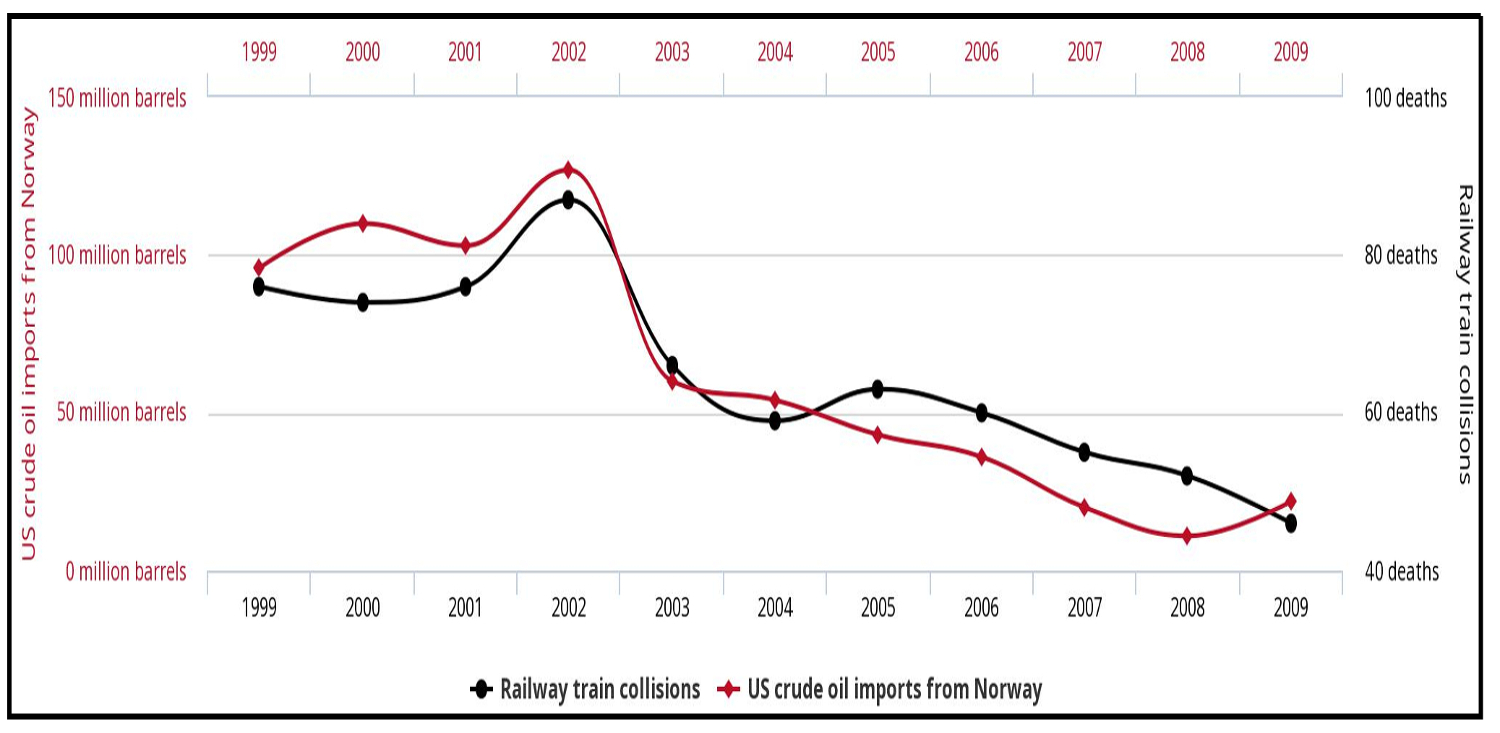
\includegraphics[angle=0, scale=0.250]{figure.jpeg}
\caption{Inserir a legenda da figura, sem ponto final}
\label{fig1}
\end{figure}

O estilo das bordas das tabelas é livre. Uma linha em branco deve ser inserida acima e abaixo de cada figura ou tabela.

\begin{table}[!h]
\centering
\caption{Resultados experimentais para propriedades de flexão de compósitos CFRC-4HS e CFRC-TWILL.  \protect\\Amplitude/profundidade razão = 35: 1. Resultados médios de 7 espécimes.}
\begin{tabular}{|c|c|c|}
\hline
Composite Properties & CFRC-TWILL & CFRC-4HS\\
\hline
Flexural Strength (MPa)$^{(1)}$ & 209$\pm$ 10 & 180 $\pm$  15\\
\hline
Flexural Modulus (GPa)$^{(1)}$ & 57.0 $\pm$ 2.8 & 18.0 $\pm$  1.3\\
\hline
Mid-span deflection at the failure stress (mm) & 2.15 $\pm$  1.90 & 6.40 $\pm$  0.25\\
\hline
\end{tabular}
\\
\begin{tabular}{p{11cm}ll}
$^{(1)}$ medido a 25$^{o}$C & &
\end{tabular}
\
\label{tab1}
\end{table}

\section{AGRADECIMENTOS}
Esta seção, opcional, deve ser posicionada antes da lista de referências.

\section{REFERÊNCIAS} 

A lista de referências deve ser introduzida como uma nova seção, localizada ao final do artigo. A primeira linha de cada referência deve ser alinhada à esquerda e as outras linhas devem ter recuo de 0,5 cm da margem esquerda. Todas as referências incluídas nesta seção devem ter sido mencionadas no texto.

As referências devem ser organizadas em ordem alfabética, de acordo com o último nome do primeiro autor. Veja os seguintes exemplos

\bibliographystyle{abcm}
\renewcommand{\refname}{}
\bibliography{bibfile}

\section{RESPONSABILIDADE PELAS INFORMAÇÕES}

Os autores são os únicos responsáveis pelas informações incluídas neste trabalho.

\end{document}
